%%%%%%%%%%%%%%%%%%%%%%%%%%%%%%%%%%%%%%%%%
% Présentation Beamer - Modifications Logicielles ALPR
% Évolutions de l'Interface Web et du Serveur Backend
%%%%%%%%%%%%%%%%%%%%%%%%%%%%%%%%%%%%%%%%%

\documentclass[
	11pt,
	aspectratio=169,
]{beamer}

\graphicspath{{Images/}{./}}

\usepackage{booktabs}
\usepackage{amsmath}
\usepackage[utf8]{inputenc}
\usepackage[T1]{fontenc}

%----------------------------------------------------------------------------------------
%	THÈME ET CONFIGURATION
%----------------------------------------------------------------------------------------

\usetheme{Madrid}
\useinnertheme{circles}
\usepackage[default]{opensans}
\usepackage{palatino}

%----------------------------------------------------------------------------------------
%	INFORMATIONS DE LA PRÉSENTATION
%----------------------------------------------------------------------------------------

\title[ALPR - Modifications]{Système RAPI : Évolutions Logicielles}
\subtitle{Interface Web, Backend et Applications Mobiles}

\author[Équipe IA]{Membres de l'Équipe du laboratoire}

\institute[UATM]{
	UATM GASA FORMATION\\
	\smallskip
	\textit{info@uatm-gasa.com}
}

\date[\today]{\today}

%----------------------------------------------------------------------------------------

\begin{document}

%----------------------------------------------------------------------------------------
%	PAGE DE TITRE
%----------------------------------------------------------------------------------------

\begin{frame}
	\titlepage
\end{frame}

%----------------------------------------------------------------------------------------
%	TABLE DES MATIÈRES
%----------------------------------------------------------------------------------------

\begin{frame}
	\frametitle{Les grandes Lignes}
	\tableofcontents
\end{frame}

%----------------------------------------------------------------------------------------
%	MODIFICATIONS INTERFACE WEB
%----------------------------------------------------------------------------------------

\section{Évolutions de l'Interface Web}

\begin{frame}
	\frametitle{Modernisation de l'Interface Web}
	\framesubtitle{Migration et Restructuration}
	
	\begin{block}{Mise à niveau technologique}
		\begin{itemize}
			\item \textbf{Migration Chakra UI V2 $\rightarrow$ V3} : Adoption des dernières fonctionnalités et optimisations
			\item \textbf{Restructuration architecturale} : Réorganisation modulaire du code pour une meilleure maintenabilité
		\end{itemize}
	\end{block}
	
	\bigskip
	
	\begin{exampleblock}{Avantages}
		\begin{itemize}
			\item Code plus propre et modulaire
			\item Performance améliorée
			\item Facilité de maintenance et d'évolution
		\end{itemize}
	\end{exampleblock}
\end{frame}

%------------------------------------------------

\begin{frame}
	\frametitle{Nouvelles Fonctionnalités Utilisateur (1/2)}
	
	\begin{columns}[t]
		\begin{column}{0.48\textwidth}
			\begin{block}{Visualisation Améliorée}
				\textbf{Détails d'analyse}
				\begin{itemize}
					\item Accès aux détails post-analyse
					\item Informations complètes sur les détections
				\end{itemize}
				
				\bigskip
				
				\textbf{Visualiseur d'images}
				\begin{itemize}
					\item Zoom avant/arrière
					\item Navigation sur images
					\item Inspection détaillée des résultats
				\end{itemize}
			\end{block}
		\end{column}
		
		\begin{column}{0.48\textwidth}
			\begin{block}{Indicateurs Visuels}
				\textbf{Niveau de confiance}
				\begin{itemize}
					\item \textcolor{green}{Vert} : Haute confiance
					\item \textcolor{orange}{Jaune} : Confiance moyenne
					\item \textcolor{red}{Rouge} : Faible confiance
				\end{itemize}
				
				\bigskip
				
				\alert{Interface intuitive et informative}
			\end{block}
		\end{column}
	\end{columns}
\end{frame}

%------------------------------------------------

\begin{frame}
	\frametitle{Nouvelles Fonctionnalités Utilisateur (2/2)}
	
	\begin{block}{Intégration Backend et Multimédia}
		\begin{itemize}
			\item \textbf{Synchronisation Backend} : Intégration complète des mises à jour API
			\item \textbf{Support audio} : Analyse de plaques sur clips audio avec appréciation de la qualité
		\end{itemize}
	\end{block}
	
	\bigskip
	
	\begin{exampleblock}{Optimisation UX/UI}
		\textbf{Audit complet réalisé sur :}
		\begin{itemize}
			\item Performance de l'interface
			\item Expérience utilisateur (UX)
			\item Meilleur accessibilité
		\end{itemize}
	\end{exampleblock}
\end{frame}

%------------------------------------------------

\begin{frame}
	\frametitle{Visuel d'Interface Web (1/2)}
	
	\begin{figure}
		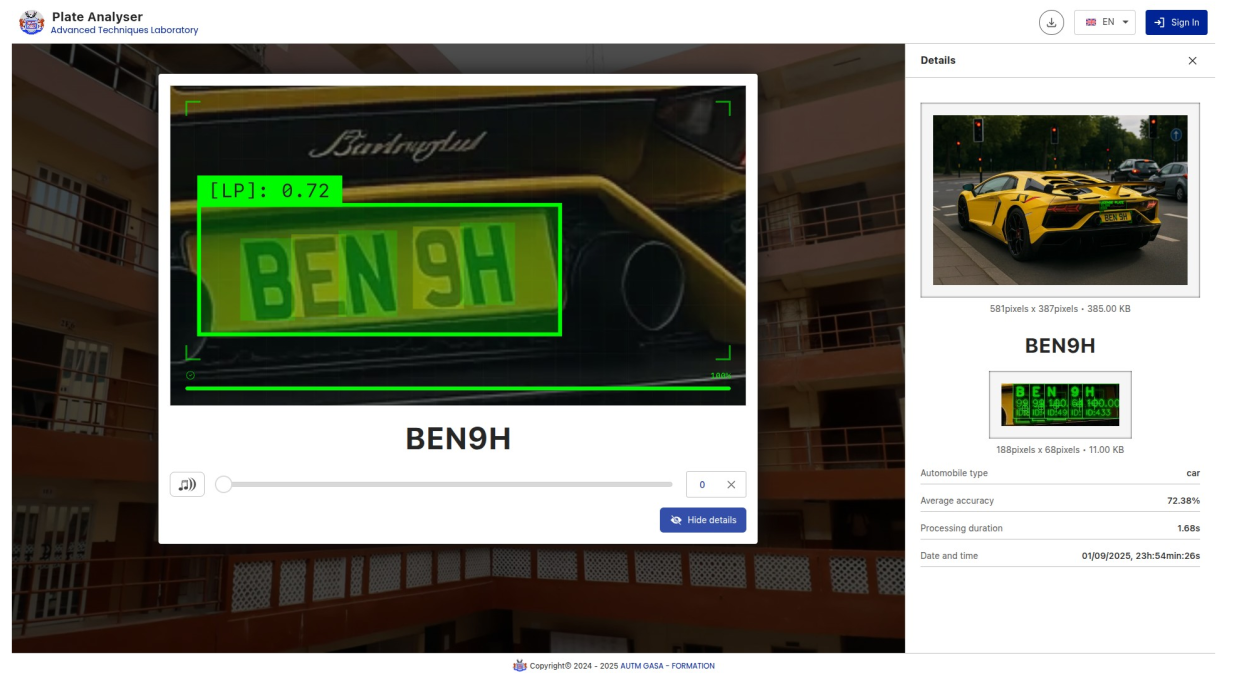
\includegraphics[width=0.9\linewidth]{Images/image1.png}
		\caption{Interface Web}
	\end{figure}
\end{frame}

%------------------------------------------------

\begin{frame}
	\frametitle{Visuel d'Interface Web (2/2)}
	
	\begin{figure}
		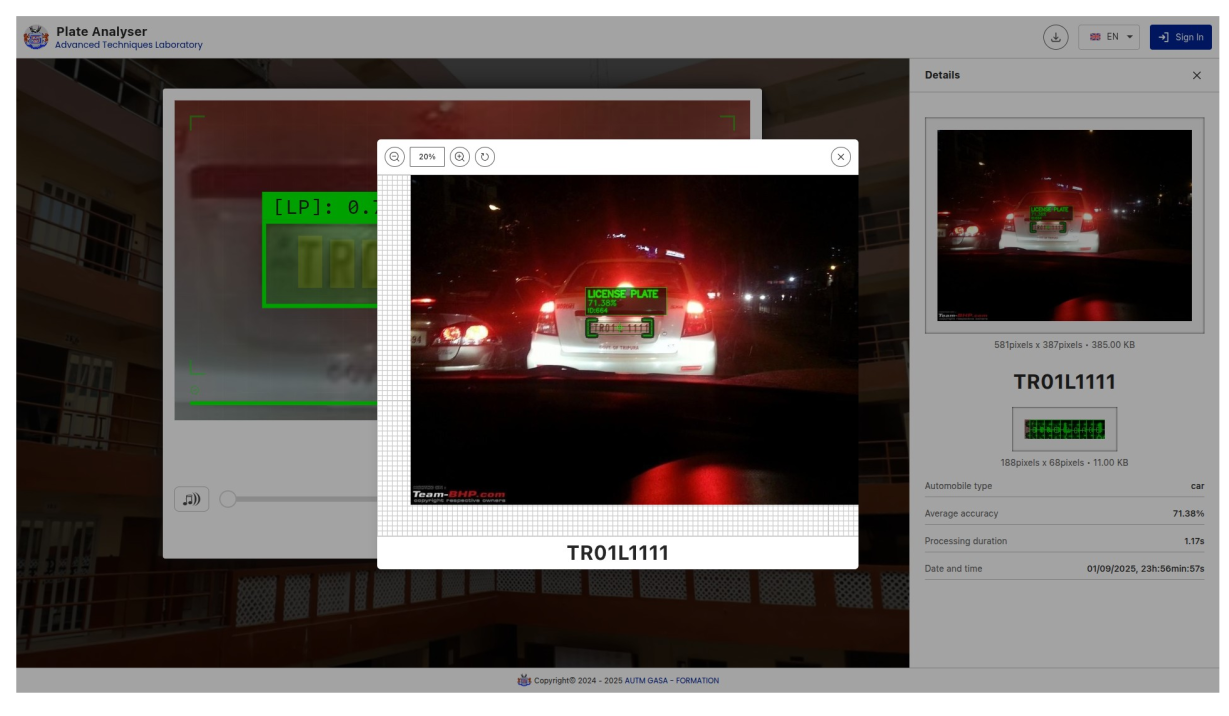
\includegraphics[width=0.9\linewidth]{Images/image2.png}
		\caption{Interface Web}
	\end{figure}
\end{frame}


%------------------------------------------------

%----------------------------------------------------------------------------------------
%	MODIFICATIONS APPLICATION MOBILE
%----------------------------------------------------------------------------------------

\section{Application Mobile Android}

\begin{frame}
	\frametitle{Mise à Niveau de l'Application Android}
	
	\begin{block}{Évolutions majeures}
		\begin{itemize}
			\item Adaptation aux nouvelles fonctionnalités du serveur
			\item Version web de l'application Android mise à jour
		\end{itemize}
	\end{block}
	
	% \bigskip
	
	% \begin{alertblock}{Résultat}
	% 	Application mobile plus performante et alignée avec le Backend
	% \end{alertblock}
\end{frame}

%----------------------------------------------------------------------------------------
%	MODIFICATIONS BACKEND
%----------------------------------------------------------------------------------------

\section{Refactoring du Backend (FastAPI)}

\begin{frame}
	\frametitle{Refactoring Complet du Backend}
	\framesubtitle{Architecture RESTful Optimisée}
	
	\begin{block}{Restructuration des Endpoints}
		\textbf{Avant :} Un seul endpoint monolithique exécutant tout le pipeline
		
		\bigskip
		
		\textbf{Après :} Endpoints atomiques avec fonctionnalités spécifiques
	\end{block}
	
	\smallskip
	
	\begin{exampleblock}{Avantages de l'approche atomique}
		\begin{itemize}
			\item \textbf{Granularité} : Exécution de fonctionnalités spécifiques
			sans le pipeline complet
			\item \textbf{Performance} : Réduction des appels inutiles
			\item \textbf{Flexibilité} : Le frontend peut composer ses propres
			workflows
			\item \textbf{Scalabilité} : Meilleure gestion de la charge serveur
			et facilité d'intégration de nouvelles endpoints
		\end{itemize}
	\end{exampleblock}
\end{frame}

%------------------------------------------------

\begin{frame}
	\frametitle{Amélioration du Traitement d'Images}
	
	\begin{block}{Algorithme de Correction de Pixels}
		\textbf{Problème identifié :}
		\begin{itemize}
			\item Images uploadées avec des défauts de pixels
			\item Risque de mauvaises détections
		\end{itemize}

		\smallskip
		
		\textbf{Solution implémentée :}
		\begin{itemize}
			\item Algorithme de correction des pixels intégré au pipeline
			\item Prétraitement automatique des images
			% \item Amélioration de la qualité avant analyse
		\end{itemize}
	\end{block}
	
	\smallskip
	
	\begin{alertblock}{Impact}
		Réduction significative des erreurs dues à la qualité d'image
	\end{alertblock}
\end{frame}

%----------------------------------------------------------------------------------------
%	SYSTÈME DE CORRECTION DES PLAQUES
%----------------------------------------------------------------------------------------

\section{Système de Correction Intelligente}

\begin{frame}
	\frametitle{Problématique : Confusions Visuelles}
	\framesubtitle{Lettres et Chiffres Similaires}
	
	\begin{alertblock}{Le Problème}
		Le modèle IA peut confondre des caractères visuellement similaires
	\end{alertblock}
	
	\begin{block}{Solution}
		\centering
		\alert{Correcteur automatique} basé sur les conventions béninoises
	\end{block}
\end{frame}

%------------------------------------------------

\begin{frame}
	\frametitle{Problématique : Confusions Visuelles}
	\framesubtitle{Exemple de confusion}

	\begin{exampleblock}{Exemple Concret}
		\textbf{Plaque réelle :} \texttt{BN0684}
		
		\textbf{Détection IA :} \texttt{8N06BA}
		
		\smallskip
		
		\textbf{Confusions identifiées :}
		\begin{itemize}
			\item \texttt{B} confondu avec \texttt{8}
			\item \texttt{8} confondu avec \texttt{B}
			\item \texttt{4} confondu avec \texttt{A}
		\end{itemize}
	\end{exampleblock}
	
\end{frame}

%------------------------------------------------

\begin{frame}
	\frametitle{Conventions des Plaques au Bénin}
	\framesubtitle{Formats Standards}
	
	\begin{columns}[t]
		\begin{column}{0.48\textwidth}
			\begin{block}{Motos}
				\textbf{Format 1 :}
				\begin{itemize}
					\item 1 chiffre
					\item 2 lettres
					\item 4 chiffres
				\end{itemize}
				\centering
				\texttt{1AB2345}
				
				\smallskip
				
				\textbf{Format 2 :}
				\begin{itemize}
					\item 1 chiffre
					\item 1 lettre
					\item 4 chiffres
				\end{itemize}
				\centering
				\texttt{1A2345}
			\end{block}
		\end{column}
		
		\begin{column}{0.48\textwidth}
			\begin{block}{Voitures}
				\textbf{Format 1 :}
				\begin{itemize}
					\item 2 lettres
					\item 4 chiffres
				\end{itemize}
				\centering
				\texttt{AB1234}
				
				\smallskip
				
				\textbf{Format 2 :}
				\begin{itemize}
					\item 1 lettre
					\item 4 chiffres
				\end{itemize}
				\centering
				\texttt{A1234}
			\end{block}
		\end{column}
	\end{columns}
	
	\bigskip
	
	\begin{alertblock}{Base du système de correction}
		Ces conventions permettent de déterminer si un caractère devrait être une lettre ou un chiffre
	\end{alertblock}
\end{frame}

%------------------------------------------------

\begin{frame}
	\frametitle{Algorithme de Correction (1/2)}
	\framesubtitle{Table de Confusion}
	
	\begin{block}{Composants du Système}
		\begin{itemize}
			\item \textbf{chiffre\_db} : Base de données des chiffres (0-9)
			\item \textbf{lettre\_db} : Base de données des lettres (A-Z)
			\item \textbf{table\_confusion} : Dictionnaire des correspondances
		\end{itemize}
	\end{block}
	
	\smallskip
	
	\begin{exampleblock}{Table de Confusion (Exemples)}
		\small
		\begin{tabular}{ccccccccc}
			\texttt{0 $\rightarrow$ O/D} & \texttt{1 $\rightarrow$ I} & \texttt{2 $\rightarrow$ Z} & \texttt{5$\rightarrow$S} & \texttt{6$\rightarrow$G} & \texttt{7$\rightarrow$T} & \texttt{8$\rightarrow$B} & ...
		\end{tabular}
	\end{exampleblock}

\end{frame}

%------------------------------------------------

\begin{frame}
	\frametitle{Algorithme de Correction (2/2)}
	\framesubtitle{Logique de Traitement}
	
	\begin{block}{Processus de Correction}
		\begin{enumerate}
			\item Vérifier le nombre de caractères détectés
			\item Comparer avec le format attendu (moto/voiture)
			\item Si confusion détectée : consulter la table et corriger
			\item Si caractères en excès : supprimer le surplus
		\end{enumerate}
	\end{block}
\end{frame}


%------------------------------------------------

\begin{frame}
	\frametitle{Logique de Correction : Étapes Détaillées}
	
	\begin{block}{Étape 1 : Validation du Format}
		\begin{itemize}
			\item Vérifier que le nombre de caractères correspond aux conventions
			\item Identifier le type de véhicule (moto ou voiture)
		\end{itemize}
	\end{block}
	
	\smallskip
	
	\begin{block}{Étape 2 : Correction Position par Position}
		Pour chaque position dans la plaque :
		\begin{itemize}
			\item \textbf{Si lettre attendue + chiffre détecté} $\rightarrow$ Remplacer par lettre correspondante
			\item \textbf{Si chiffre attendu + lettre détectée} $\rightarrow$ Remplacer par chiffre correspondant
		\end{itemize}
	\end{block}
	
	\smallskip
	
	\begin{alertblock}{Gestion des Cas Particuliers}
		\begin{itemize}
			\item Caractères en excès : Suppression automatique
			\item Format non conforme : Tentative de reconstruction
		\end{itemize}
	\end{alertblock}
\end{frame}

%------------------------------------------------

\begin{frame}
	\frametitle{Exemple de Correction en Action}
	\framesubtitle{Cas d'une Voiture}
	
	\begin{columns}[c]
		\begin{column}{0.48\textwidth}
			\begin{block}{Détection Brute}
				\Large
				\centering
				\texttt{8N06BA}
				
				\normalsize
				\bigskip
				
				\textbf{Problèmes :}
				\begin{itemize}
					\item Position 1 : \textcolor{red}{\texttt{8}} (chiffre)
					\item Position 5 : \textcolor{red}{\texttt{B}} (lettre)
					\item Position 6 : \textcolor{red}{\texttt{A}} (lettre)
				\end{itemize}
			\end{block}
		\end{column}
		
		\begin{column}{0.48\textwidth}
			\begin{exampleblock}{Après Correction}
				\Large
				\centering
				\textcolor{green}{\texttt{BN0684}}
				
				\normalsize
				\bigskip
				
				\textbf{Corrections :}
				\begin{itemize}
					\item \texttt{8} $\rightarrow$ \textcolor{green}{\texttt{B}} (lettre)
					\item \texttt{B} $\rightarrow$ \textcolor{green}{\texttt{8}} (chiffre)
					\item \texttt{A} $\rightarrow$ \textcolor{green}{\texttt{4}} (chiffre)
				\end{itemize}
			\end{exampleblock}
		\end{column}
	\end{columns}
	
	\smallskip
	
	\begin{block}{Format Respecté}
		\centering
		Voiture : \texttt{[Lettre][Lettre][Chiffre][Chiffre][Chiffre][Chiffre]}
	\end{block}
\end{frame}

%------------------------------------------------

\begin{frame}
	\frametitle{Impact et Bénéfices du Correcteur}
	
	\begin{exampleblock}{Amélioration de la Précision}
		\begin{itemize}
			\item Correction automatique des confusions visuelles
			\item Respect strict des conventions béninoises
			\item Réduction des faux positifs
		\end{itemize}
	\end{exampleblock}
	
	\smallskip
	
	\begin{block}{Avantages Opérationnels}
		\begin{itemize}
			\item \textbf{Robustesse} : Gère les erreurs de détection courantes
			\item \textbf{Adaptabilité} : Facile d'ajouter de nouvelles règles
			\item \textbf{Traçabilité} : Possibilité de logger les corrections
		\end{itemize}
	\end{block}
	
	\smallskip
	
	\begin{alertblock}{Résultat}
		\centering
		Le correcteur améliore significativement la fiabilité du système
		en transformant les détections ambiguës en résultats conformes
	\end{alertblock}
\end{frame}

%----------------------------------------------------------------------------------------
%	CONDITIONS DE FONCTIONNEMENT
%----------------------------------------------------------------------------------------

\section{Conditions de Fonctionnement du Modèle}

\begin{frame}
	\frametitle{Spécifications Techniques du Modèle}
	\framesubtitle{Contraintes et Limitations}
	
	\begin{alertblock}{Exigences de Résolution}
		Résolution minimale requise : $1280 \times 720$ ou $720 \times 1280$ pixels
	\end{alertblock}

	\begin{block}{Conditions de Capture}
		\begin{enumerate}
			\item \textbf{Distance maximale} : 12 mètres entre la caméra et la plaque
			
			\item \textbf{Angle de prise de vue} : Entre 45° et 90°
			\begin{itemize}
				\item Ne pas photographier depuis le sol en pointant vers le haut
				\item \alert{Interdiction de prise du haut} (aucun dataset disponible)
			\end{itemize}
		\end{enumerate}
	\end{block}
\end{frame}

%------------------------------------------------

\begin{frame}
	\frametitle{Limitations du Modèle}
	
	\begin{alertblock}{Cas de Non-Fonctionnement}
		Le modèle \alert{ne peut pas} détecter les plaques suivantes :
		\begin{itemize}
			\item Plaques trop rouillées
			\item Plaques anciennes avec numéros effacés
			\item Plaques en mauvais état général
		\end{itemize}
	\end{alertblock}
	
	\bigskip
	
	\begin{exampleblock}{Recommandations}
		Pour des résultats optimaux :
		\begin{itemize}
			\item Éclairage suffisant (dans la journée est mieux)
			\item Plaques en bon état
			\item Respect des angles et distances
			\item Résolution d'image adéquate
		\end{itemize}
	\end{exampleblock}
\end{frame}

%----------------------------------------------------------------------------------------
%	SCHÉMA RÉCAPITULATIF
%----------------------------------------------------------------------------------------

\begin{frame}
	\frametitle{Récapitulatif : Conditions Optimales}
	
	\begin{table}
		\centering
		\begin{tabular}{lc}
			\toprule
			\textbf{Paramètre} & \textbf{Valeur / Condition} \\
			\midrule
			Résolution minimale & $1280 \times 720$ px \\
			Distance maximale & 12 mètres \\
			Angle de prise de vue & 45° -- 90° \\
			État de la plaque & Bon (non rouillée) \\
			Prise du haut / pointant vers le haut & \textcolor{red}{Non supportée} \\
			Qualité d'image & Correction automatique activée \\
			\bottomrule
		\end{tabular}
		\caption{Spécifications techniques du système ALPR actuelle}
	\end{table}
\end{frame}

%----------------------------------------------------------------------------------------
%	SYNTHÈSE
%----------------------------------------------------------------------------------------

\section{Synthèse}

\begin{frame}
	\frametitle{Synthèse des Modifications}
	
	\begin{columns}[t]
		\begin{column}{0.32\textwidth}
			\begin{block}{Interface Web}
				\small
				\begin{itemize}
					\item Migration Chakra UI V3
					\item Visualiseur d'images
					\item Indicateurs visuels
					\item Audit UX/UI
				\end{itemize}
			\end{block}
		\end{column}
		
		\begin{column}{0.32\textwidth}
			\begin{block}{Backend}
				\small
				\begin{itemize}
					\item Endpoints atomiques pour optimiser les appels
					\item Correction pixels
					\item Correction automatique des numéros lus
				\end{itemize}
			\end{block}
		\end{column}
		
		\begin{column}{0.32\textwidth}
			\begin{block}{Mobile}
				\small
				\begin{itemize}
					\item Mise à niveau de l'application Android avec le nouveau
					endpoint de téléversement
					% \item Nouvel envoi images
					% \item Synchronisation
					% \item Performance
				\end{itemize}
			\end{block}
		\end{column}
	\end{columns}
	
	\bigskip\bigskip
	
	\begin{exampleblock}{Résultat Global}
		\centering
		Écosystème logiciel modernisé, performant et évolutif
	\end{exampleblock}
\end{frame}

%----------------------------------------------------------------------------------------
%	PERSPECTIVES
%----------------------------------------------------------------------------------------

\section{Sécurité et Perspectives}

\begin{frame}
	\frametitle{Prochaines Évolutions : Sécurisation}
	
	\begin{block}{Authentification API}
		\textbf{Implémentation prévue :} Système d'authentification JWT
		
		\bigskip
		
		\textbf{Objectifs :}
		\begin{itemize}
			\item Sécuriser l'accès aux endpoints
			\item Gestion des clés API
			\item Traçabilité des requêtes
			% \item Limitation du taux d'utilisation (rate limiting)
		\end{itemize}
	\end{block}
	
	\smallskip
	
	\begin{exampleblock}{Bénéfices attendus}
		\begin{itemize}
			\item Protection contre les accès non autorisés
			% \item Gestion commerciale des licences
			\item Monitoring des utilisations
		\end{itemize}
	\end{exampleblock}
\end{frame}


%----------------------------------------------------------------------------------------
%	COMPARAISON AVANT/APRÈS
%----------------------------------------------------------------------------------------

\begin{frame}
	\frametitle{Comparaison Avant/Après}
	
	\begin{table}
		\centering
		\small
		\begin{tabular}{lcc}
			\toprule
			\textbf{Aspect} & \textbf{Avant} & \textbf{Après} \\
			\midrule
			Interface UI & Chakra UI V2 & \textcolor{green}{Chakra UI V3} \\
			Architecture Frontend & Monolithique & \textcolor{green}{Modulaire} \\
			Endpoints Backend & Unique & \textcolor{green}{Atomiques} \\
			Qualité d'image & Brute & \textcolor{green}{Corrigée} \\
			Visualisation & Basique & \textcolor{green}{Avancée + Zoom} \\
			Confiance IA & Non visible & \textcolor{green}{Couleurs} \\
			% Support Audio & Pas d'appréciation & \textcolor{green}{Ap} \\
			Sécurité API & Basique & \textcolor{orange}{JWT (prévu)} \\
			\bottomrule
		\end{tabular}
	\end{table}
	
	\bigskip
	
	\centering
	\alert{Évolution majeure de l'ensemble de la plateforme}
\end{frame}



%----------------------------------------------------------------------------------------
%	CONCLUSION
%----------------------------------------------------------------------------------------

\begin{frame}
	\frametitle{Conclusion}
	
	\begin{block}{Accomplissements}
		\begin{itemize}
			\item Modernisation complète de l'écosystème logiciel
			\item Architecture backend optimisée et flexible
			\item Interface utilisateur intuitive et performante
			\item Support multiplateforme (Web + Android) pour les testes manuels
			\item Système de Correction Intelligente pour la résolution
			des confusions Visuelles
		\end{itemize}
	\end{block}
	
	\smallskip
	
	\begin{exampleblock}{Prochaine Étape Majeure}
		\centering
		Implémentation de l'authentification JWT pour sécuriser l'accès
	\end{exampleblock}
	
	\smallskip
	
	\begin{alertblock}{Vision}
		\centering
		Plateforme ALPR professionnelle, sécurisée et prête pour la production
	\end{alertblock}
\end{frame}



%----------------------------------------------------------------------------------------
%	QUESTIONS
%----------------------------------------------------------------------------------------

\begin{frame}[plain]
	\begin{center}
		{\Huge Questions ?}
		
		\bigskip\bigskip
		
		{\LARGE Commentaires et discussions}
		
		\bigskip\bigskip
		
		\textit{info@uatm-gasa.com}
	\end{center}
\end{frame}

%----------------------------------------------------------------------------------------

\end{document}
